% !TEX root = ../main.tex
\chapter{Supplementary Figures}\label{app:supp-figs}
Additional figures referenced in the main text are collated here for completeness.

\begin{figure}[ht]
    \centering
    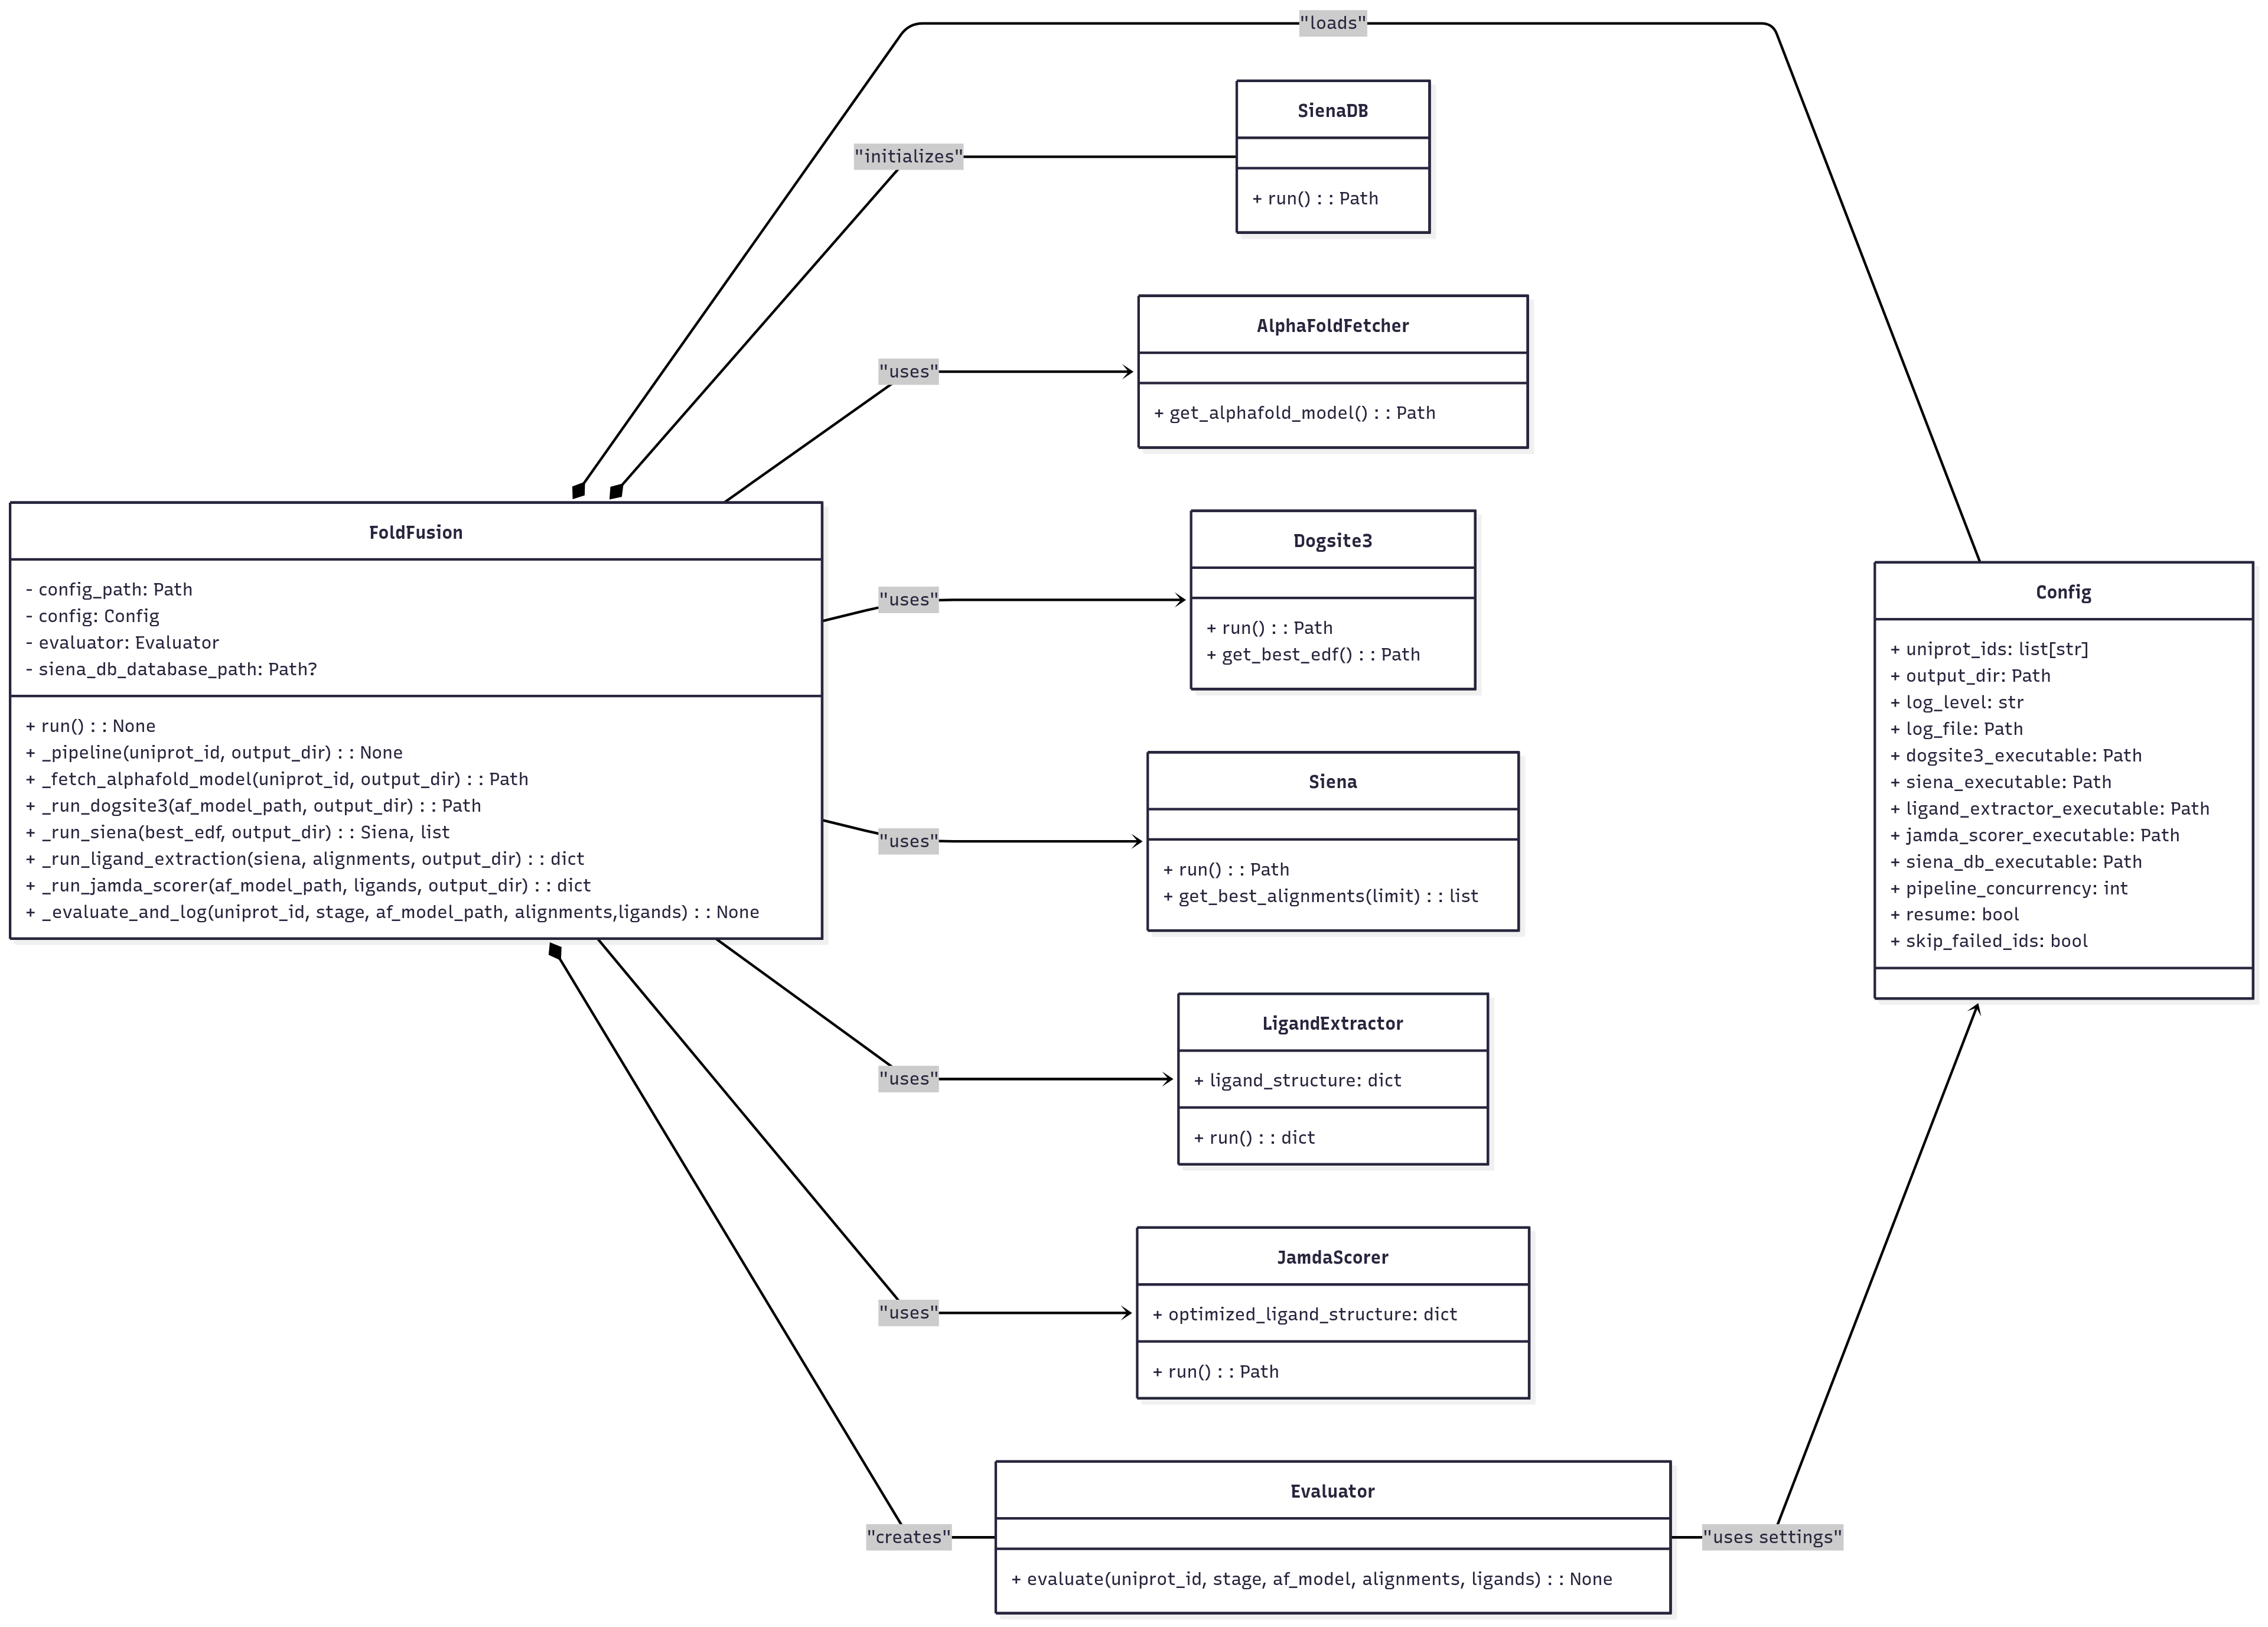
\includegraphics[width=0.95\linewidth]{figures/foldfusion_pipeline_uml.png}
    \caption[Pipeline UML overview]{UML class diagram of the pipeline. The central orchestrator coordinates data fetching, pocket detection, donor alignment, ligand extraction, scoring, and evaluation via the surrounding tool adapters and configuration object. Node labels retain the \texttt{FoldFusion} class name used in the code to denote this work's pipeline implementation.}
    \label{fig:pipeline_overview_uml}
\end{figure}

% Failure mode case studies — enlarged single-panel figures moved from main text
\begin{figure}[ht]
    \centering
    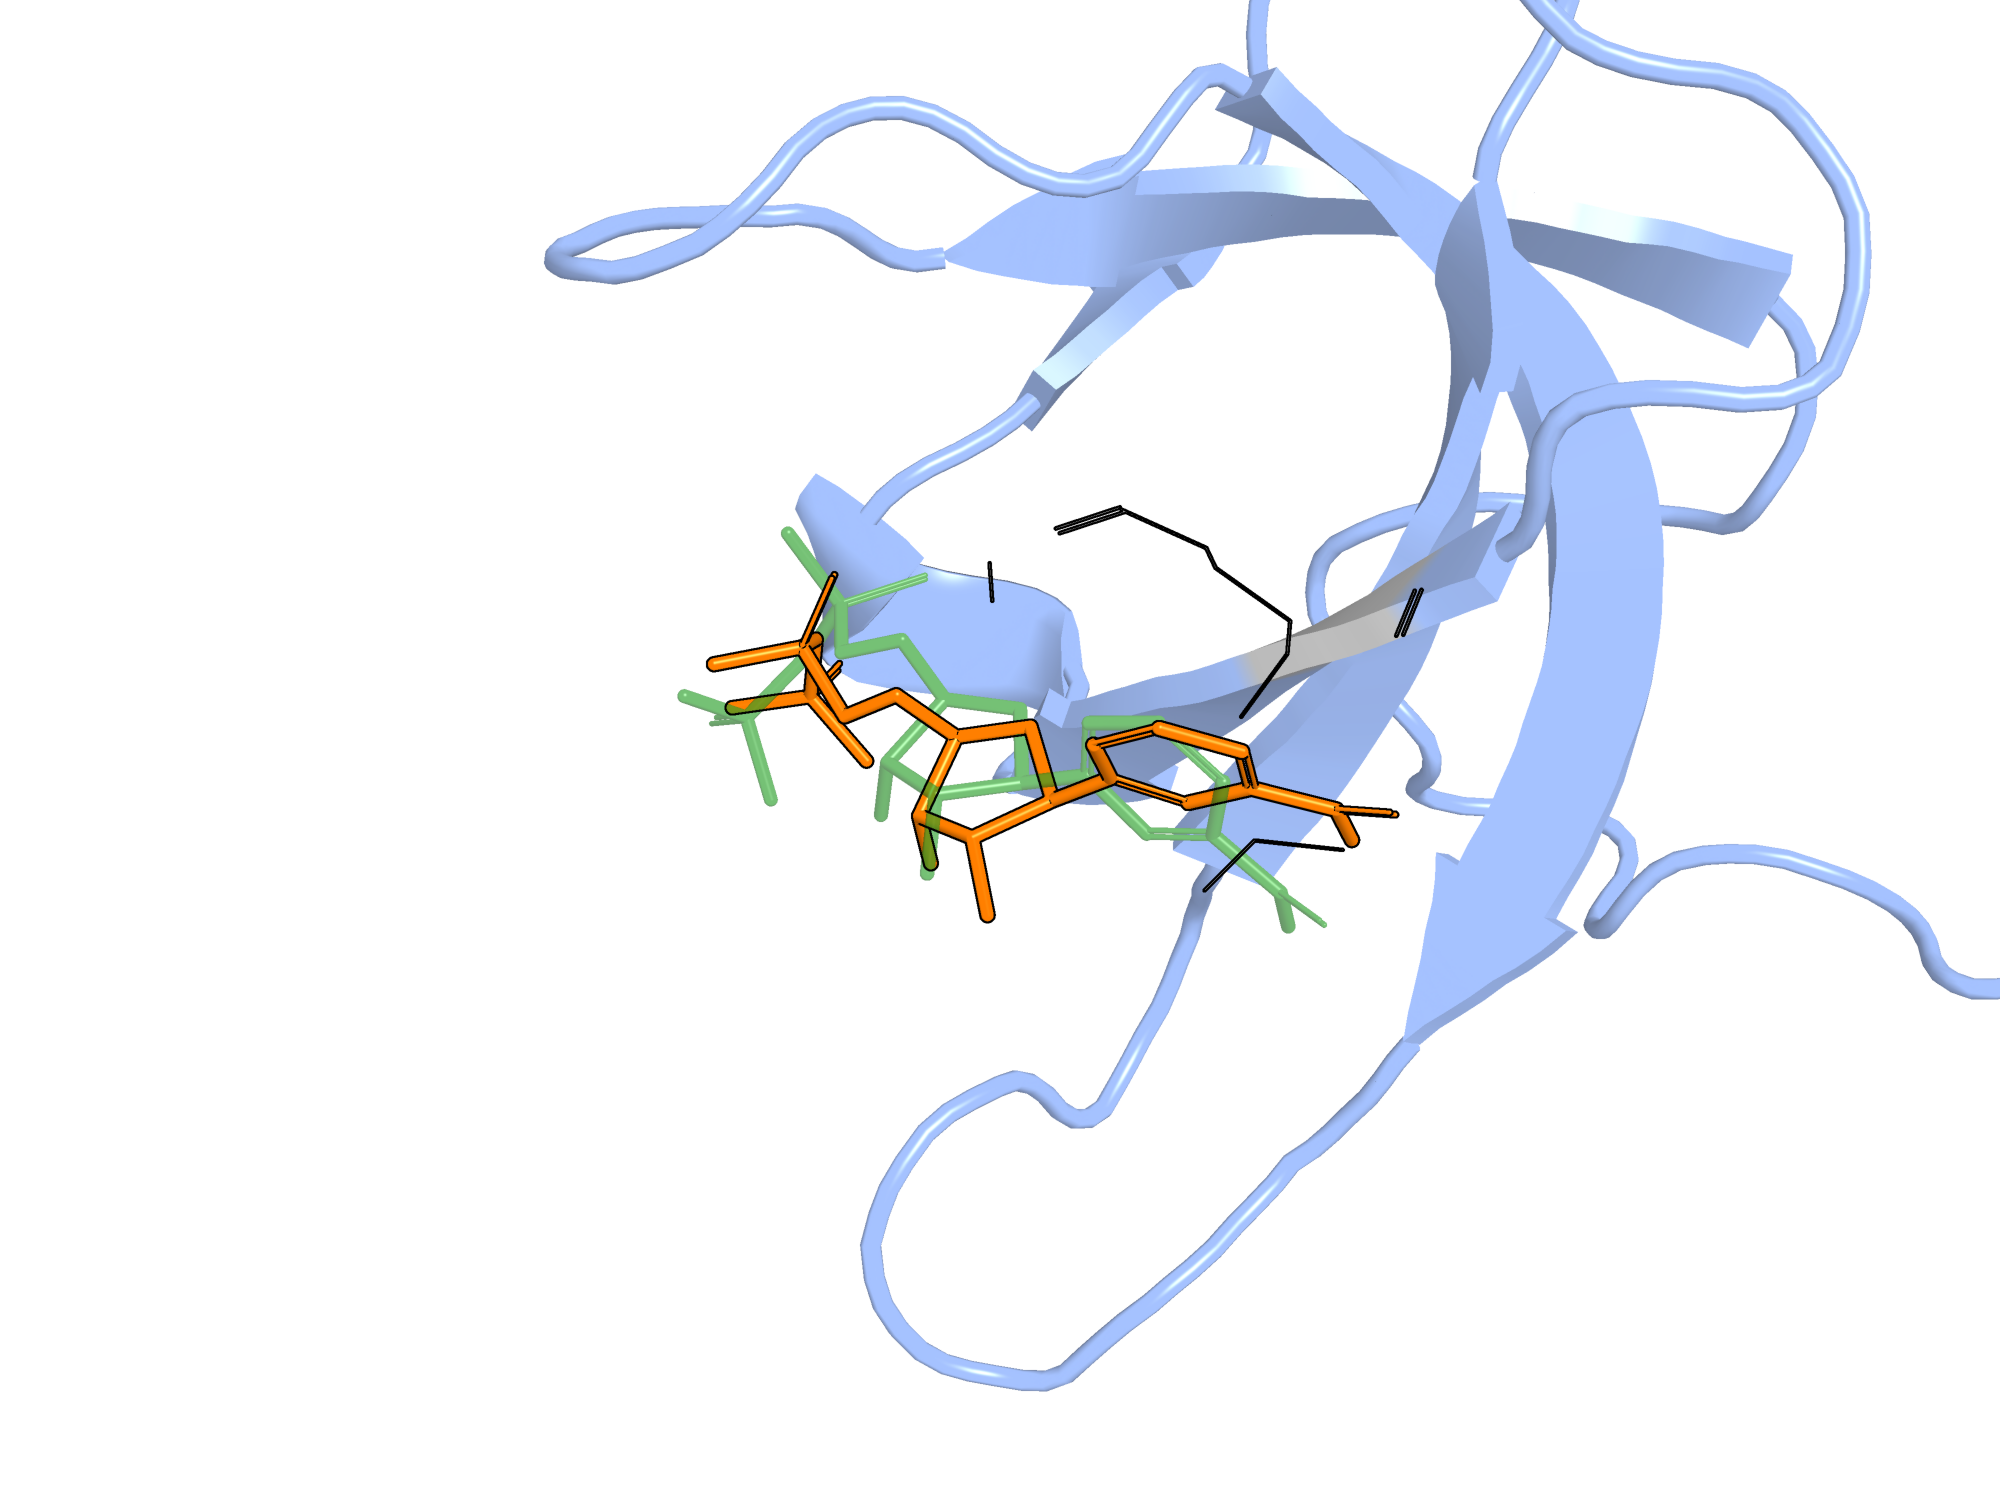
\includegraphics[width=0.85\linewidth]{figures/foldfusion_P00383_success_iso.png}
    \caption[Reference success case]{Reference success case (green: donor, orange: refined). Rendered with PyMOL~\cite{PyMOL, AxPyMOL}.}
    \label{fig:failure_modes_case_studies:success}
\end{figure}

\begin{figure}[ht]
    \centering
    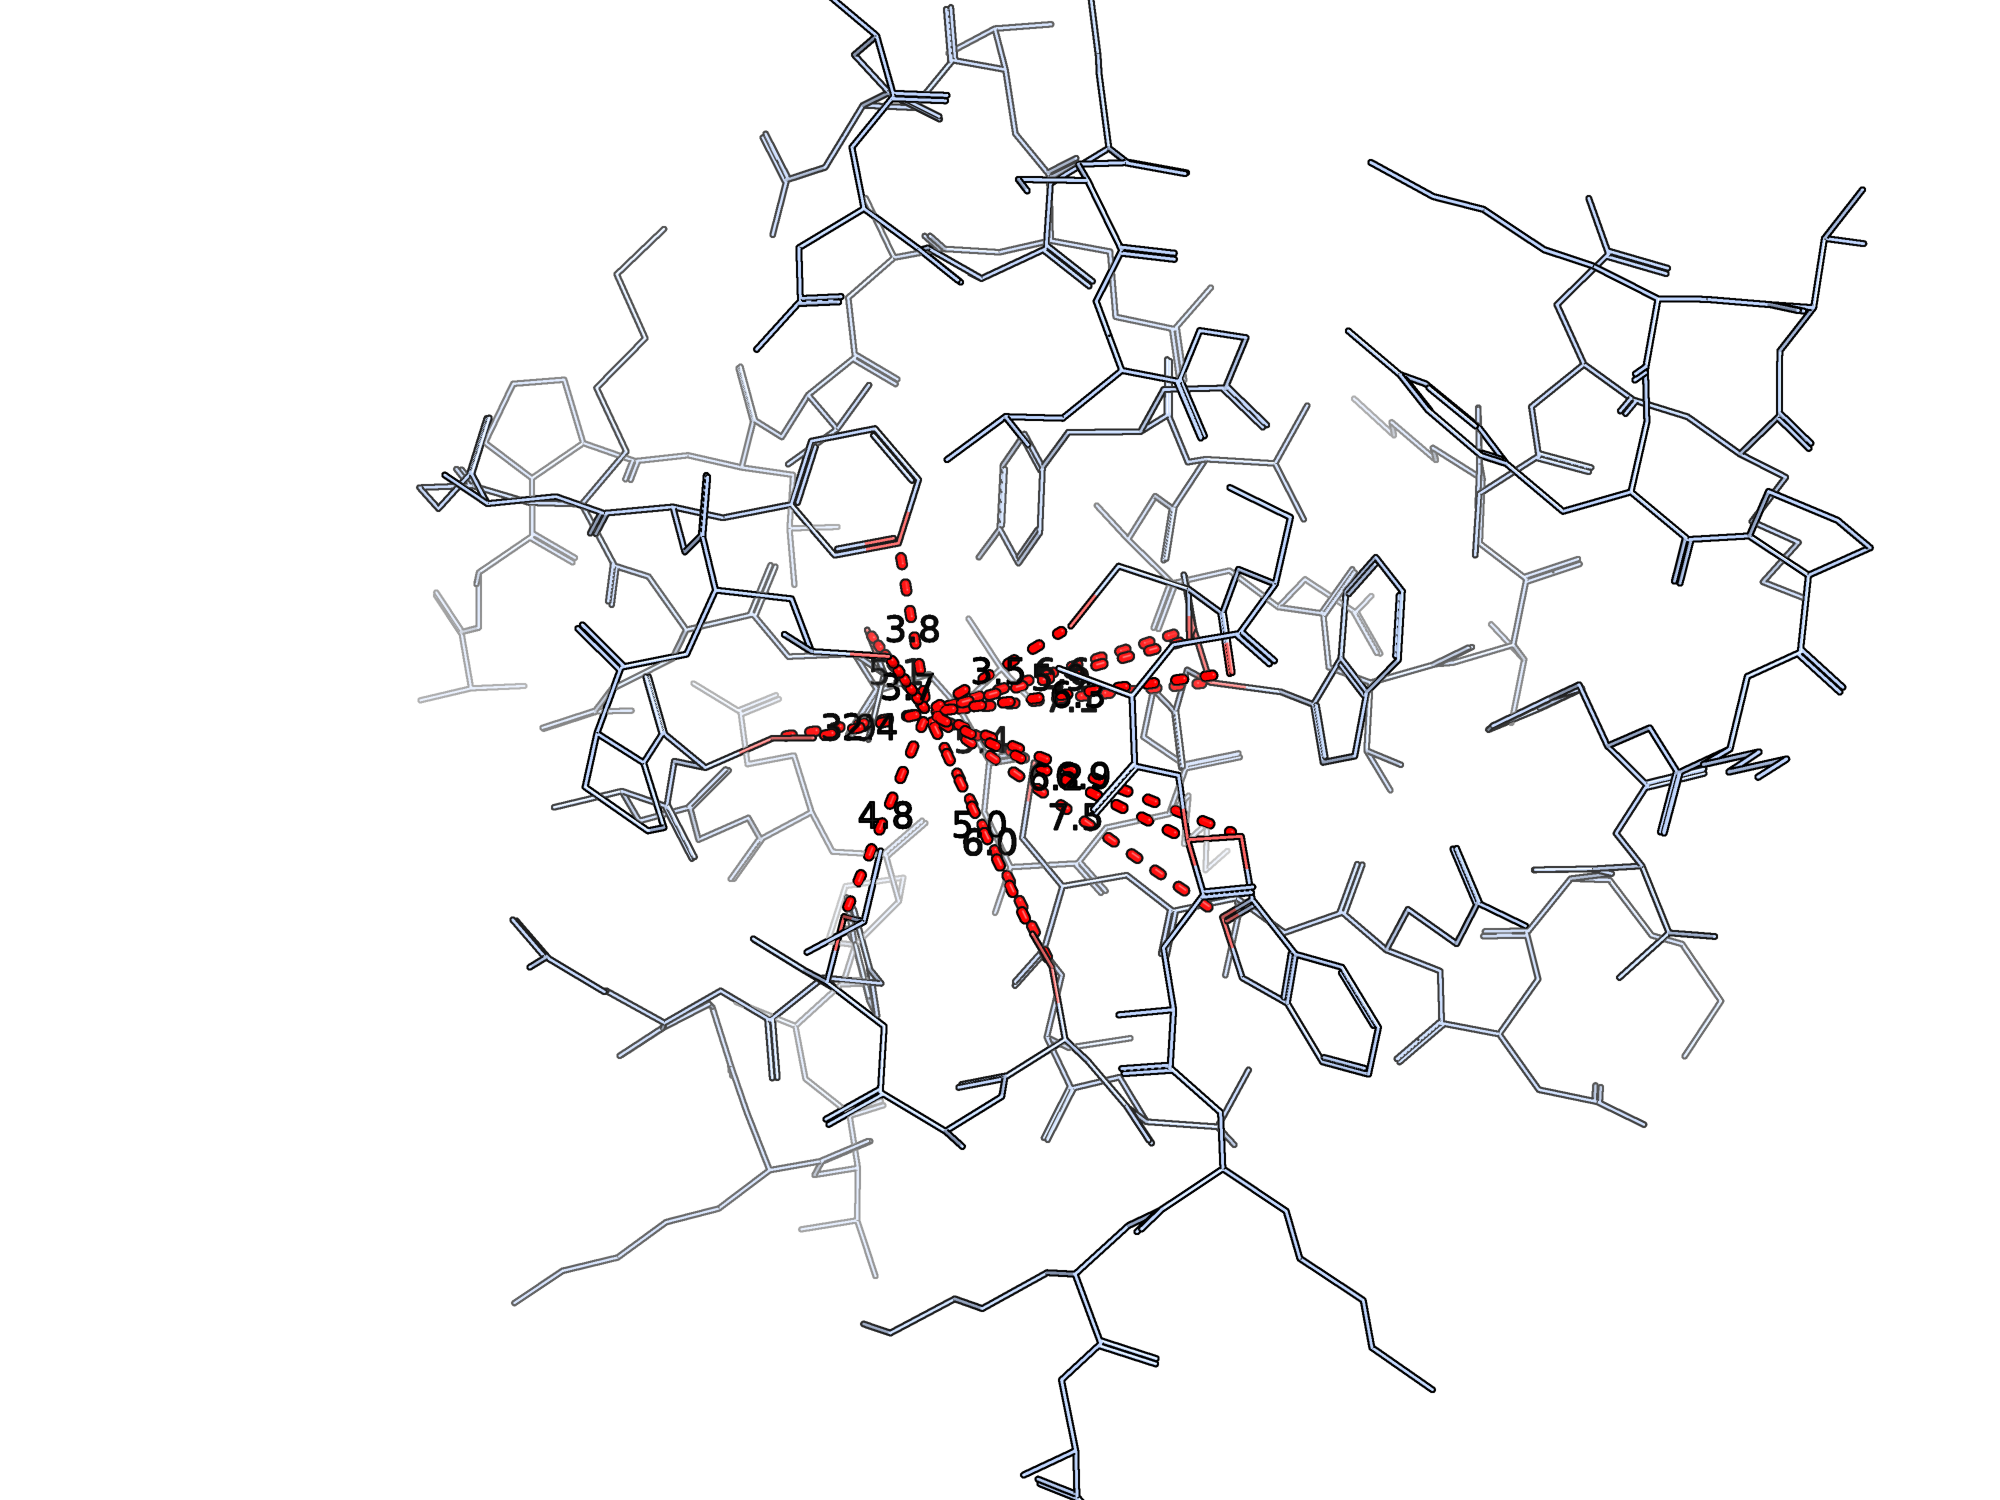
\includegraphics[width=0.85\linewidth]{figures/foldfusion_P80882_failure.png}
    \caption[Collapsed-loop failure]{Collapsed-loop failure example. Rendered with PyMOL~\cite{PyMOL, AxPyMOL}.}
    \label{fig:failure_modes_case_studies:collapsed}
\end{figure}

\begin{figure}[ht]
    \centering
    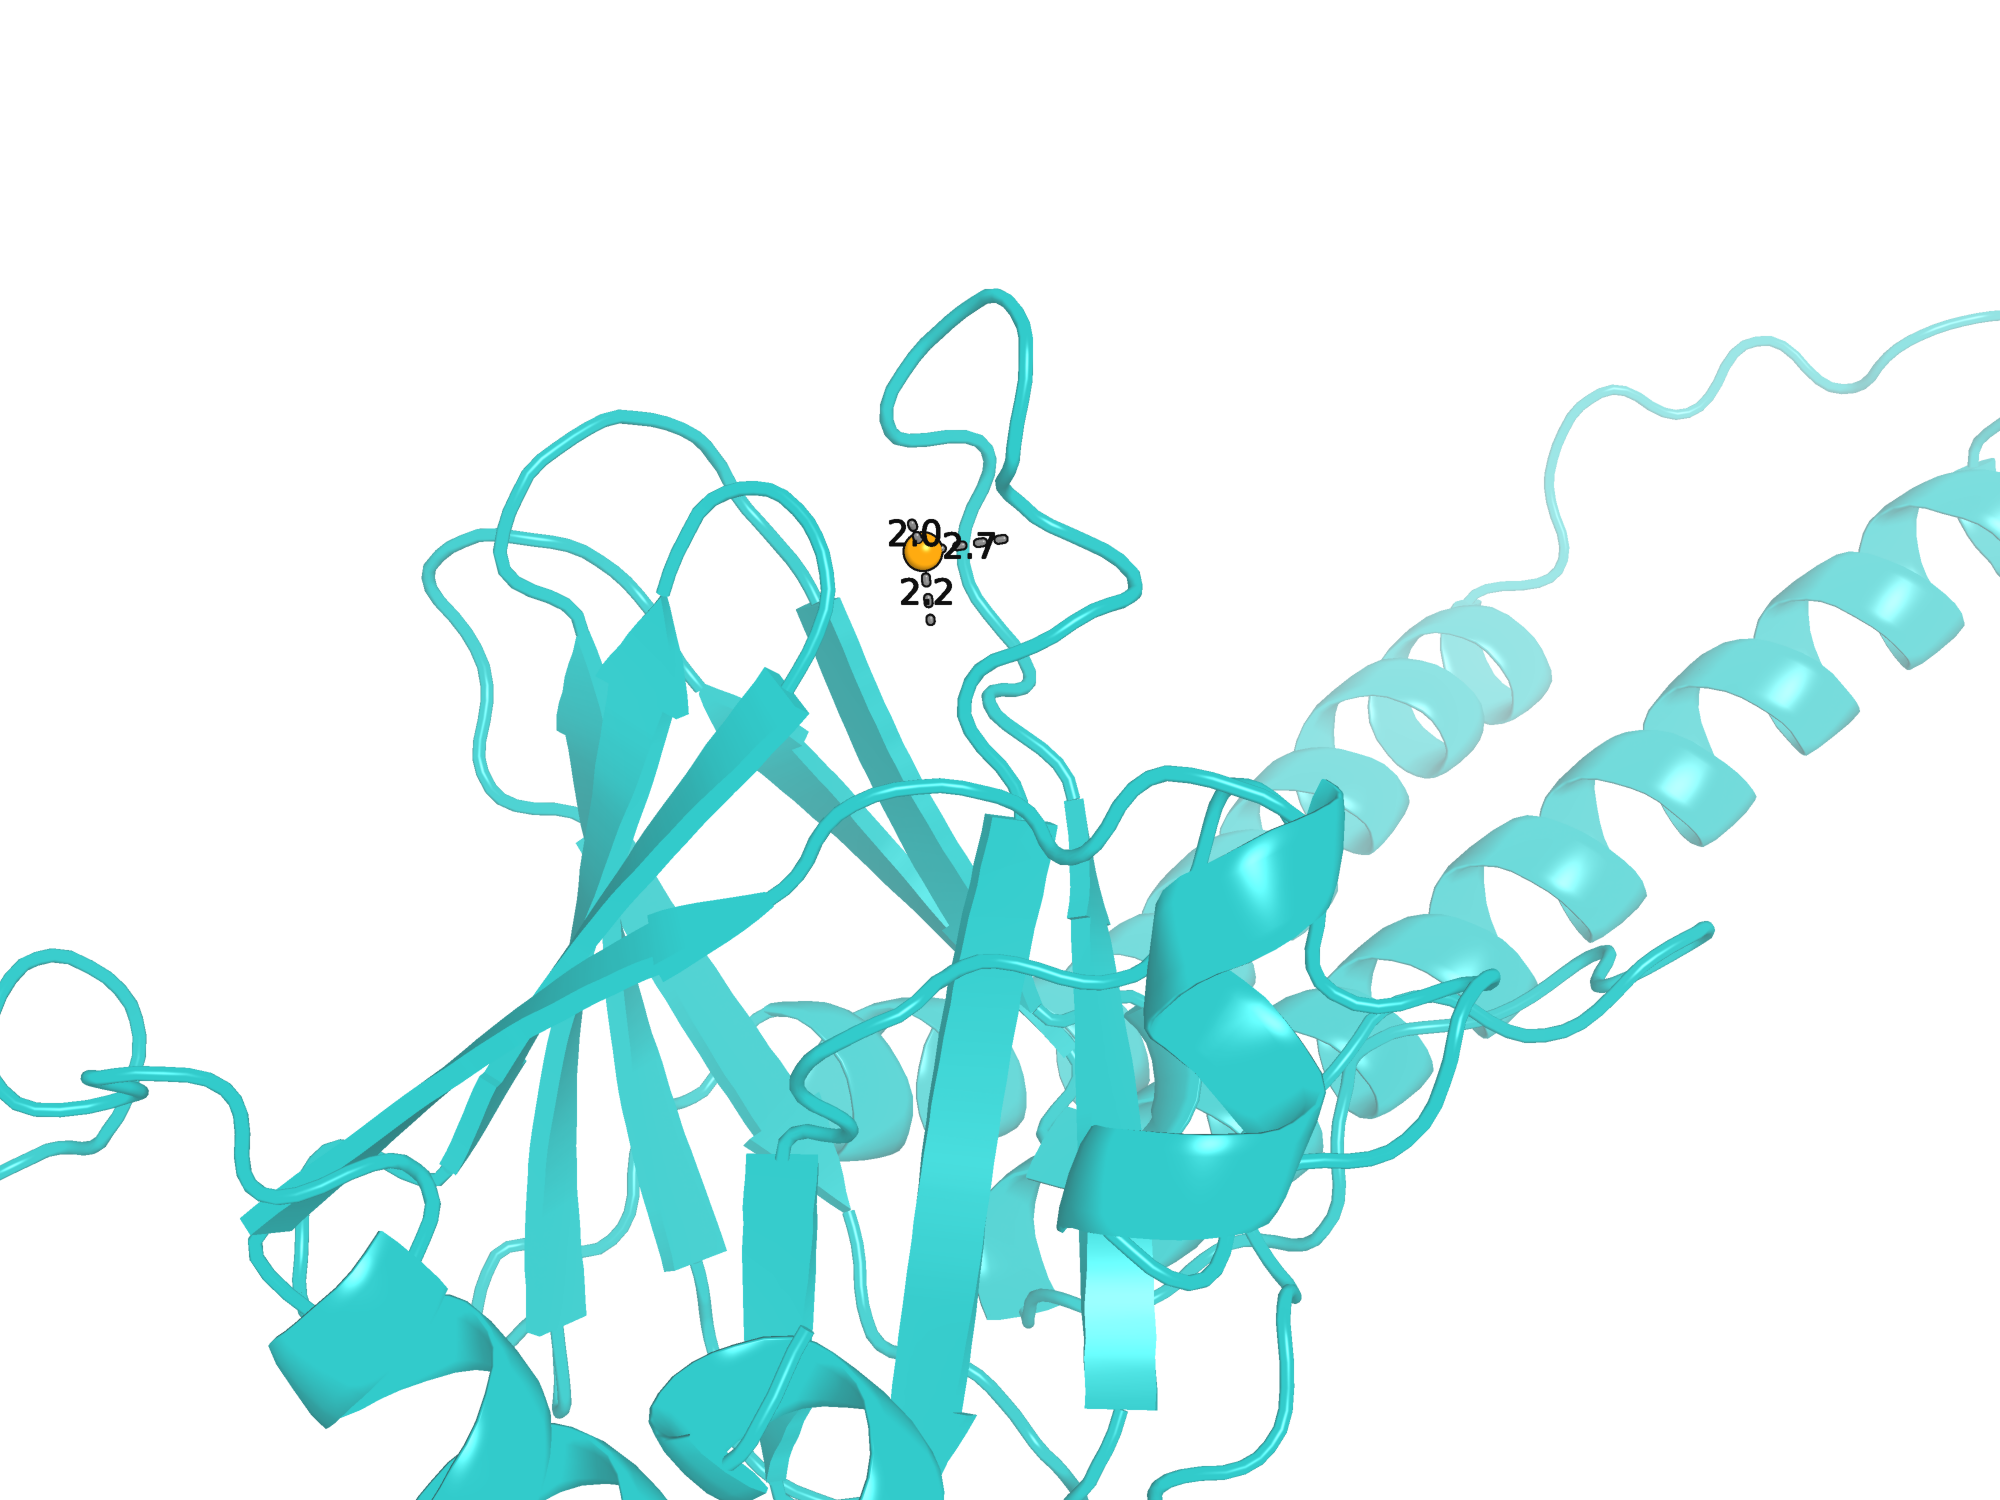
\includegraphics[width=0.85\linewidth]{figures/foldfusion_P08306_metal.png}
    \caption[Metal mis-coordination failure]{Metal mis-coordination failure example. Rendered with PyMOL~\cite{PyMOL, AxPyMOL}.}
    \label{fig:failure_modes_case_studies:metal}
\end{figure}

\begin{figure}[ht]
    \centering
    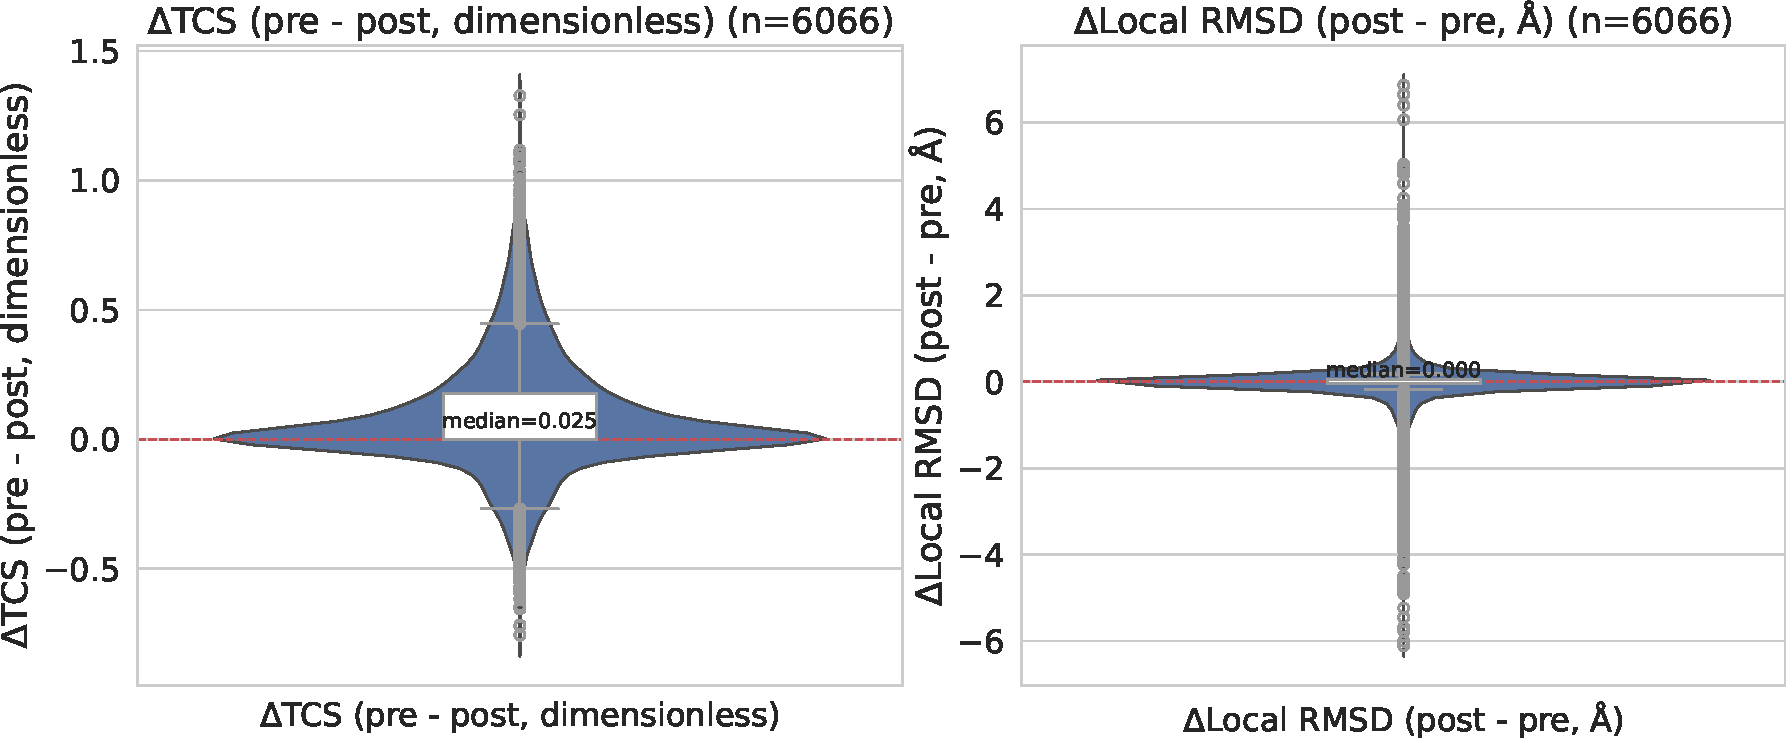
\includegraphics[width=0.85\linewidth]{figures/03_results/fig_jamda_delta_distributions.pdf}
    \caption[JAMDAscorer delta distributions]{Distributions of paired JAMDAscorer deltas ($\Delta$\gls{tcs} and $\Delta$local \gls{rmsd}) for the \num{6066} placements that produced both pre- and post-optimization metrics. Zero indicates no change, and negative $\Delta$\gls{tcs} denotes fewer clashes after optimization.}
    \label{fig:jamda-deltas}
\end{figure}

\begin{figure}[ht]
    \centering
    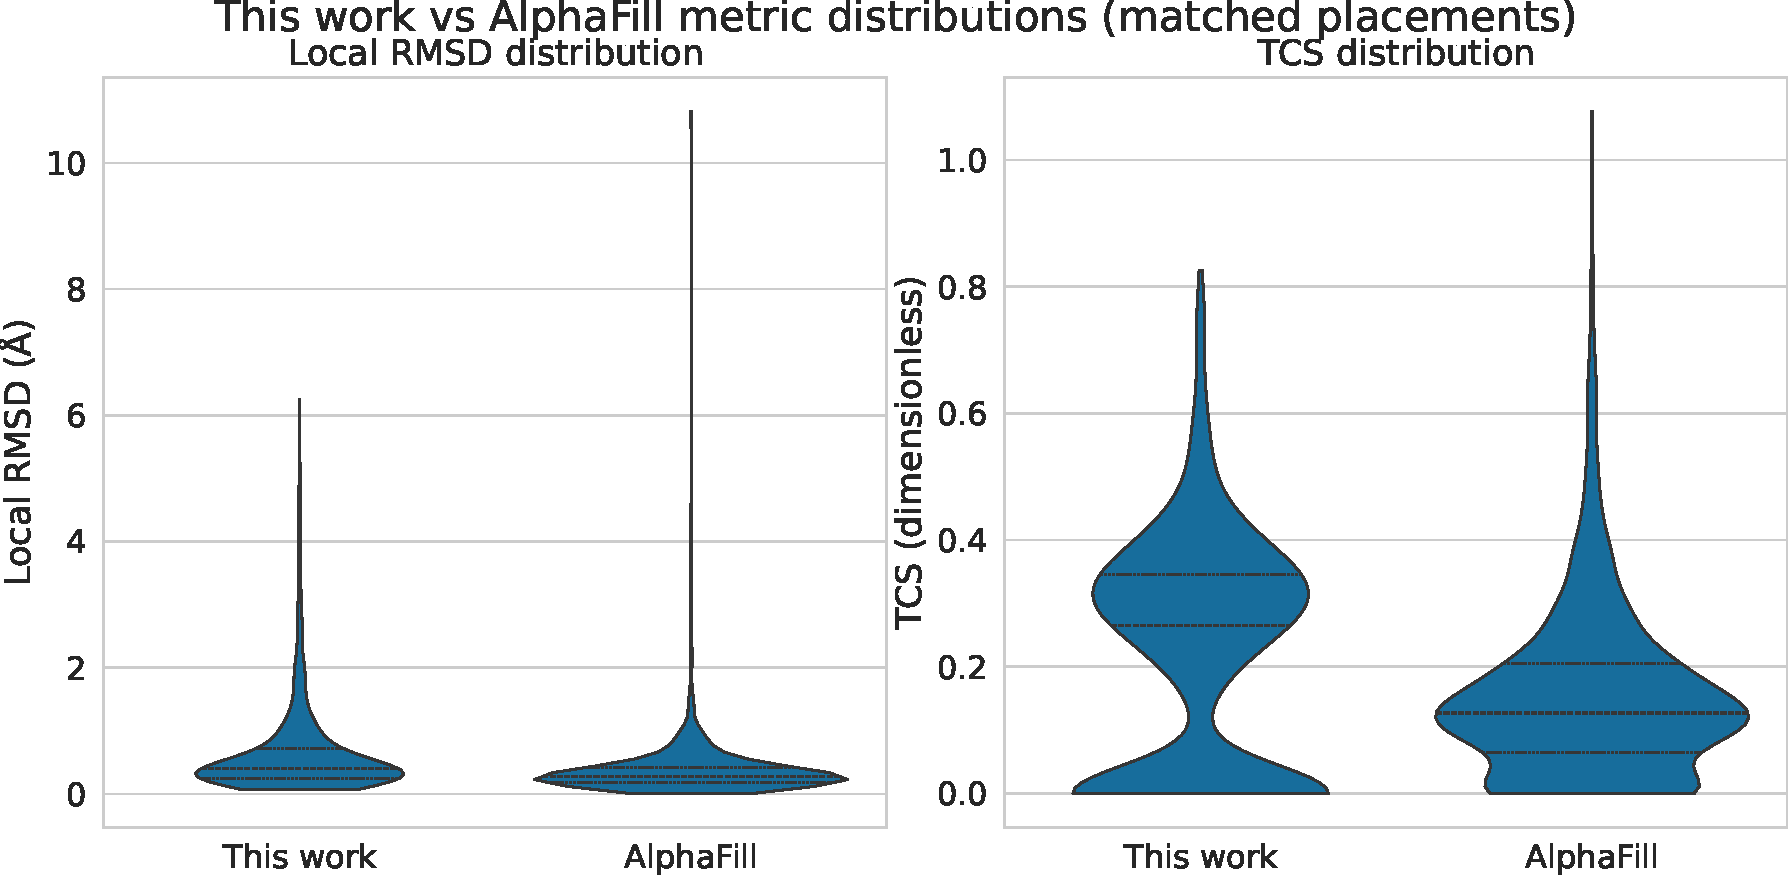
\includegraphics[width=0.9\linewidth]{figures/03_results/fig_ff_af_metric_distributions.pdf}
    \caption[Pipeline vs. AlphaFill distributions]{Distributions of local \gls{rmsd} and \gls{tcs} for this pipeline and AlphaFill on the matched cohort described in Section~\ref{sec:results-external}. Violin plots show quartiles and density for each pipeline.}
    \label{fig:ff-af-dist}
\end{figure}

\begin{figure}[ht]
    \centering
    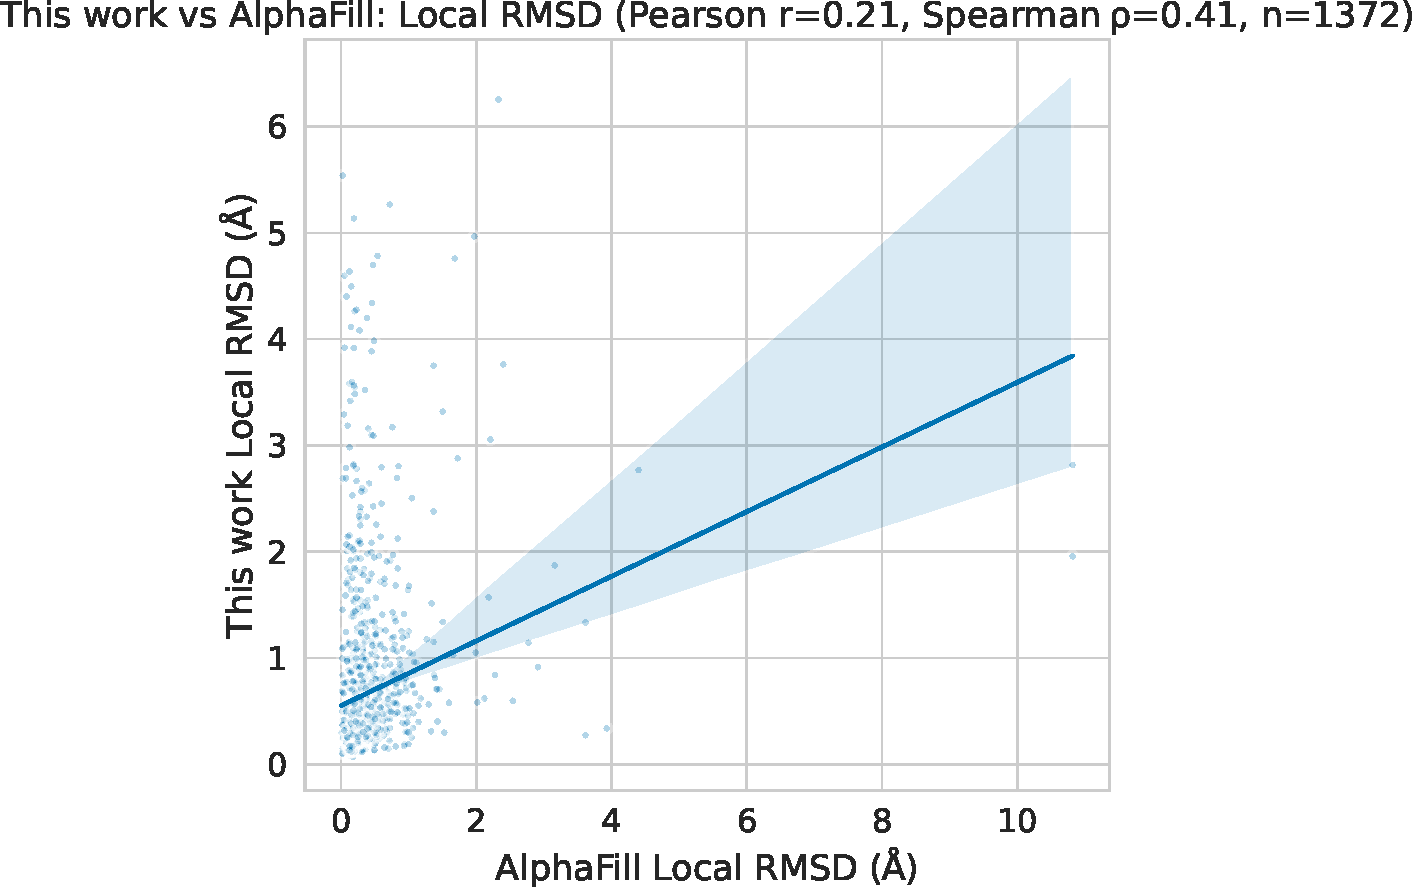
\includegraphics[width=0.49\linewidth]{figures/03_results/fig_correlation_local_rmsd_ff_vs_af.pdf}\hfill
    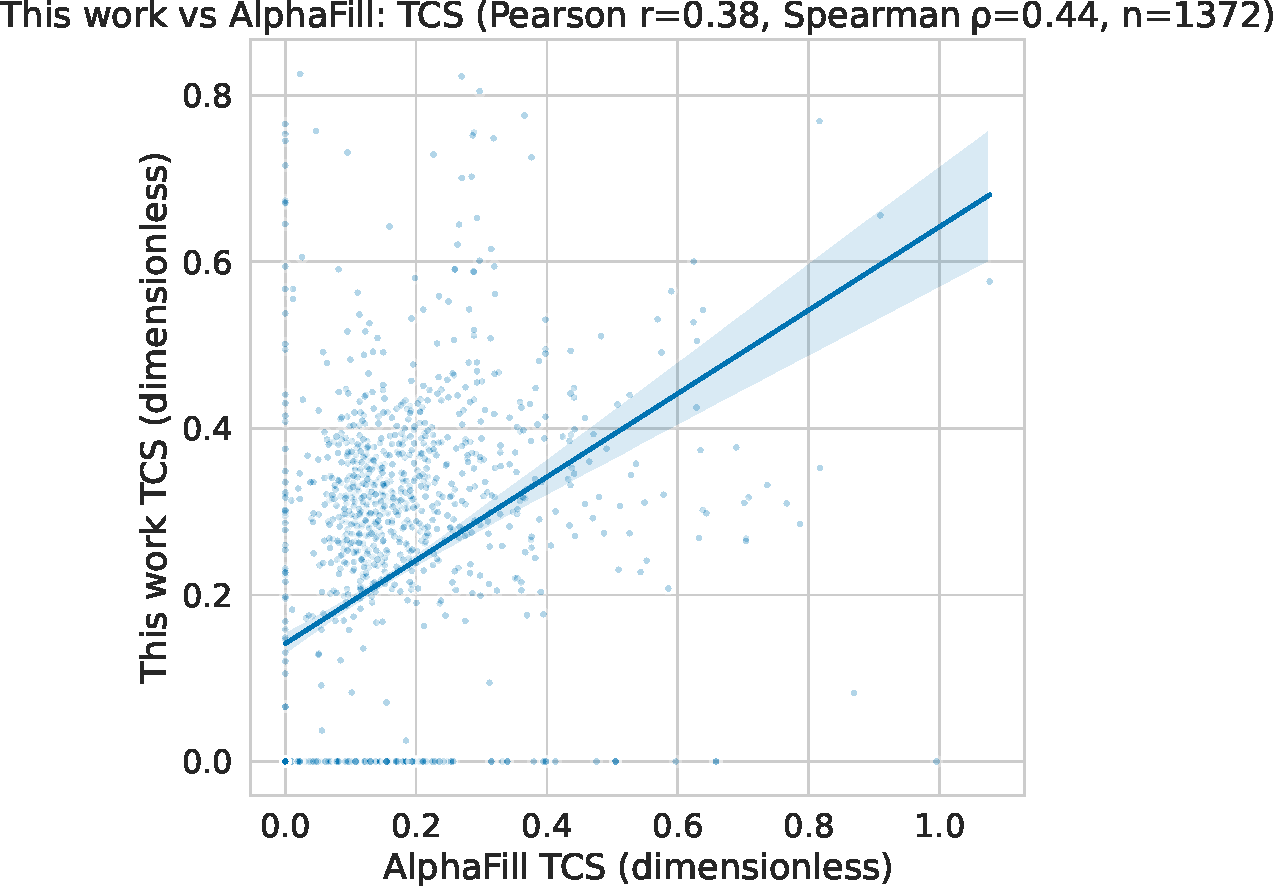
\includegraphics[width=0.49\linewidth]{figures/03_results/fig_correlation_tcs_score_ff_vs_af.pdf}
    \caption[Pipeline vs. AlphaFill correlations]{Correlation of this pipeline (TP) vs.\ AlphaFill (AF) on the matched cohort from Section~\ref{sec:results-external}. The left panel shows local \gls{rmsd} and the right panel shows \gls{tcs}; Pearson $r$ and Spearman $\rho$ with sample sizes are annotated in each title.}
    \label{fig:ff-af-corr}
\end{figure}

\begin{figure}[ht]
    \centering
    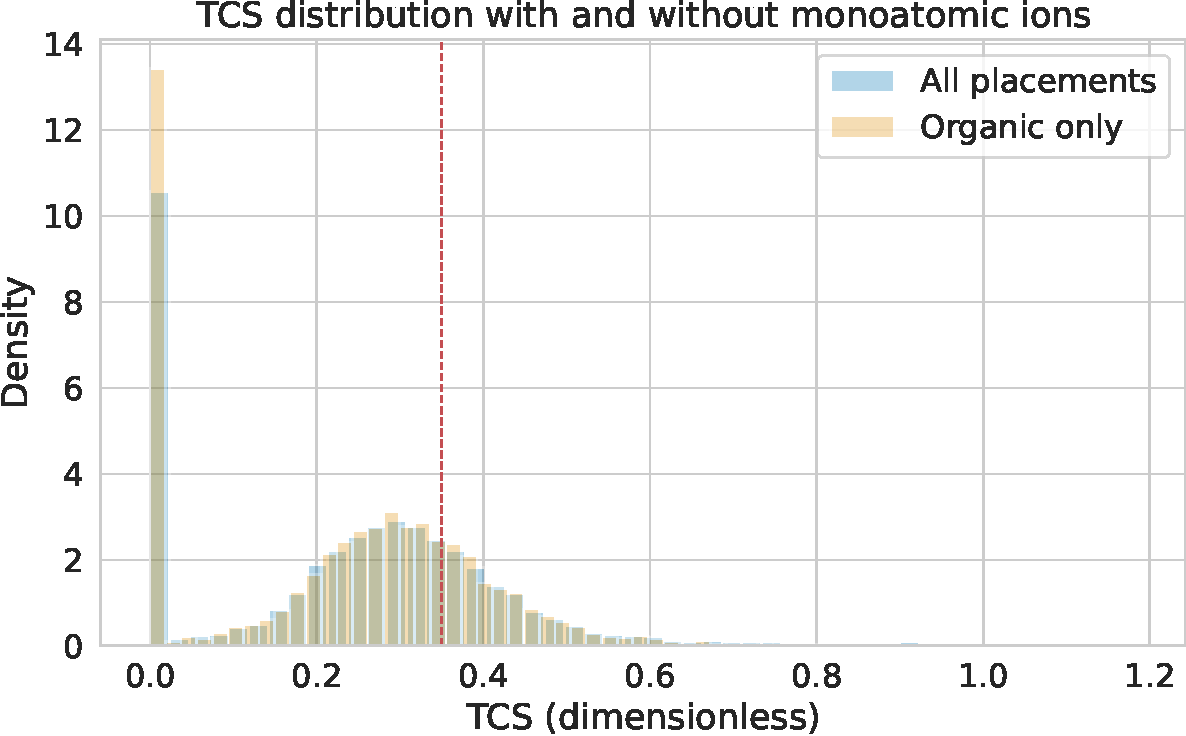
\includegraphics[width=0.75\linewidth]{figures/03_results/fig_tcs_distribution_ion_exclusion.pdf}
    \caption[TCS distributions with ion exclusion]{\gls{tcs} distributions with (blue) and without (green) monoatomic ions. The vertical line marks the \SI{0.35}{} clash threshold used throughout the analysis.}
    \label{fig:ion-exclusion}
\end{figure}
